%% LyX 2.1.3 created this file.  For more info, see http://www.lyx.org/.
%% Do not edit unless you really know what you are doing.
\documentclass[english,12pt]{infommreport}
\usepackage[T1]{fontenc}
%\usepackage[latin9]{inputenc}
\usepackage[utf8]{inputenc}
\usepackage{biblatex}
\addbibresource{BT_final_refs.bib}
\usepackage{amsmath}
\usepackage{amsfonts}
\usepackage{physics}
\usepackage{subcaption}
\makeatletter
%%%%%%%%%%%%%%%%%%%%%%%%%%%%%% User specified LaTeX commands.


%\renewcommand{\submittedtext}{A technical report for} %comment this out if you don't want to change the writing
\project{InFoMM CDT Mini-Project 1}     %the degree
\projectdate{Trinity 2018}         %the degree date
\company{BT}
\supervisors{Renaud Lambiotte, Andrew Mellor, \\
Stephen Brewis, Stephen Cassidy}%Include industrial and academic supervisors


\title{Organisational Structure}
\author{Ka Man (Ambrose) Yim}

%\makeatother

\usepackage{babel}
\begin{document}

\maketitle
\tableofcontents
\newpage
\section{Introduction}
We can think of an organisation as a problem solving machinery. A problem facing a company like Ford or BMW might be to build a certain number of cars in a month to a certain specification; the problem facing BBC is to make programmes that fit their organisational objectives to `inform, educate and entertain', subject to regulatory oversight and budget restrictions. A restaurant's problem is to make delicious food at an attractive price \emph{sans e. coli}.

The type of problems an organisation tackles are those which are too large and complex to be solved by a single person with reasonable efficiency. Hence labour is divided between many people, each person serving some function with different capabilities. This process is analogous to decomposing computations on a computer into several processes and solving them in parallel on multiple processing cores. However, unlike computer processes that execute a fixed set of instructions, humans (allegedly) have free will and agency. Thus an organisation makes its own decisions and has a life of its own through the manifold interactions and emails between people. Decision-making in organisations are rarely made in isolation by a single person. Behind each decision there is a complex web of influence and information transfer (or lack thereof). In most (if not all) levels of an organisation, decisions are reached by some form of consensus.

Should we trust humans to make decisions that best align with the global objectives of the organisation? People often fail to see beyond the costs and benefits arising from their interactions with their \emph{local} environments; few individuals have a holistic understanding of their role in the global picture of interactions. We live in a remarkable time in history (which is decidedly not at its end) when democratic decisions, entangled with advances in communication and new ways of influencing people, have shook the Western liberal-democratic political system to its core.

Nonetheless in the pre-SkyNet era, humans are the only candidates as the atoms of organisations. The question is how people should be organised to make `better' decisions. Here we present a mathematical model for decision making processes in an organisation. We assume in a corporate setting there is a well-defined `global' problem, in the sense that there is a measure to compare how well two solutions solve the same problem. A solution is a set of decisions, of which there are many.

Each person, or agent, has a decision to make. It can choose between several actions. Four characteristics fully define an agent:
\begin{enumerate}
\item the individual actions available to the agents (capabilities);
\item the bias of agents towards certain actions;
\item how actions of other agents affect an agent's bias; and
\item who the agent talks with.
\end{enumerate}
The first three features give rise to a global network describing the dependencies between agents. The position of the agent in this \textbf{dependency network} defines the influence relations between agents. The \textbf{social network} of the organisation emerges from the last feature.

Ideally, the social network of an organisation should be built around the dependency network; people whose actions are highly correlate with each other should communicate and coordinate. However, agents may not be fully aware of the full extent of the dependency network, diminishing the chance of communication between parties that influence one another. Moreover, there is a social cost involved in communication, and agents can only maintain a limited number of agents in its social sphere; thus given a sufficiently complex problem agents inevitably will fail to communicate with all of its neighbours in the dependency network.

The social network on the same level of organisational hierarchy are often structured into closely knit teams with fairly little communications between teams. In this study we study the efficiency of social networks with fairly distinct social structures in solving problems . The particular problem we are investigating is called a coordination game, where an agent only deems it desirable to coordinate if sufficiently many of its neighbours on the dependency network decide to coordinate. The global objective of the organisation is for as many agents to coordinate. This dynamics of persuasion can be mapped onto threshold contagion models on networks, where a disease or `idea' spreads along a network of people.

We want to measure how different network topologies in the communications and dependency networks influence how

We formally define our mathematical model below.

\section{Model}

We suppose there are $N$ agents working in an organisation. We follow the standard game theory agent model. Each agent $i$ has a set of actions $A_i$ and a utility function $u_i: A_1 \times \cdots A_N \to \mathbb{R}$ which assigns to each state of the system, which we define to be the collection of all the actions of the agents, a real value which we call the utility of the state to agent $i$. Given the actions of all the other agents, each agent $i$ will selfishly try to choose an action out its own set of actions $A_i$ to maximise its own utility.

In our model we assume each agent's utility is only biased by a small number of agents in the system. We construct a dependency network of influence and constraints by drawing an edge between agents whose utilities depend on one another. In our simplification we assume that inflence is reflexive i.e. $u_i  = u_i(a_i, a_j, \ldots) \Leftrightarrow u_j = u_j(a_j, a_i, \ldots)$, such that the dependency network is undirected.

As a simple model for agents adapting to new ideas in an organisation we consider the coordination game \cite{shoham_multiagent_2008} \cite{jackson_games_2014} being played out on a dependency network. In the coordination game each agent has two actions $A_i = \qty{0,1}$, where $a_i=0$ is what we call the default action and $a_i=1$ is the novel action, which represents innovation. If the agent chooses the default action $a_i=0$, the utility will always be neutral $u_i(a_i=0 \ \lvert \ a_{-i})=0$. However, if the agent elects to implement the novel action, two scenarios may arise. If a sufficiently large fraction $r_i \in [0,1]$ of its neighbours in the dependency network decide to coordinate, then the agent will receive a positive utility $u_i > 0$, and the logical action of the agent would then be to commit to the novel action. However if there are fewer than a fraction $r_i$ of neighbours in the neighbourhood to prompt the agent to innovate, the $u_i < 0$, and the best response of the agent would be return to the default action. This simple dynamic simulates the resistance to the uptake of new ideas, and the effects of constraints imposed by other agents in an organisation in deterring innnovation. We say the global objective of the organisation is to have as many agents adopt the novel action.

To characterise a population's tendency to accept new ideas, we suppose each agent samples their persuasion threshold $r_i$ from some distribution. Following Gleeson's example \cite{gleeson_seed_2007}, we suppose the distribution is a Gaussian with standard deviation $\sigma = 0.2$ and mean $R$, a parameter which we tune to adjust the characteristic of the population. Agents with $r_i<0$ will always elect to adopt new ideas. Gleeson \cite{gleeson_seed_2007} aptly refers to these agents as innovators. We need innovators to initiate the spread of $a=1$ across the population of agents. As we increase $R$, there will be fewer innovators in the population and the aggregate tolerance of new ideas is decreased.

In the case where the social network matches the dependency network, the only condition for innovation to `infect' an agent is for the agent to be exposed to sufficiently many innovative neighbours is the dependency network. However, once we decouple the social network from the dependency network, the agents need to prompted by neighbours in its social network to be aware of innovation and consider adopting it. Thus an agent is in one of three states at any time: unaware and susceptible, aware and susceptible, and aware and infected. In this regard our model is similar to the multiplex SIR contact infection models in \cite{granell_dynamical_2013}. We study two types of social interactions. In the first case, the social awareness threshold of a node, which is the smallest fraction of innovating neighbours to make a previously unaware node aware of innovation, is sampled independently from the same distribution as the depedendency threshold. This is the model studied by Lee, Brummitt and Goh \cite{lee_threshold_2014}. In the second case, an agent is aware if only one of its neighbours decides to innovate. The model we study here is a special case of the

We consider two ways which the social and dependency networks could decouple. We could take a social network and either (a) swap pairs of nodes, or (b) swap pairs of edges to obtain the dependency network (or vice versa). (a) represents the social network failing to catch up with changes in role of agents the dependency network, while (b) represents an actual change in dependency. In (a), the perturbed dependency network has the same network topology but a different correspondence between nodes between the social and dependency layers, whereas in (b) we can think of the nodes maintaing the same correspondence between layers but the network topology being altered as the two networks decouple.


The nodes update their actions according to the following rules which is widely accepted as a standard in network epidemiology literature \cite{watts_simple_2002} \cite{gleeson_seed_2007} and network game theory literature \cite{jackson_games_2014}. Firstly, the initial infected population is identified: these may be `seeds' of coordinating agents which we put in by hand, or innovators with negative thresholds. Then nodes in the $0$ state update their responses synchronously according to the information they receive and the agents whom they depend on. Once the nodes decide to innovate, they will remain in the state of innovation. We use the final fraction of infected agents $\rho$ as a measure of the success of the spread of innovation in the organisation. In our simulations we will see how $\rho$ decreases as the number of node or edge swaps increase in both (a) and (b) modes of decoupling. In our analytical study we compute the `cascade threshold', the maximal value of $R$ greater than which the population would not adopt new behaviour in the limit of infinite swaps. We compare the single layer case to the duplex social + dependency network model, and observe the influence of decoupled social awareness on the cascade of innovation.

We consider two classes of random networks. The first class are Erdős-Renyi graphs \cite{erdos_random_1959} where an edge between two nodes is present in the graph with probability $p$. The second class of networks are `planted partition models' \cite{karrer_stochastic_2011}, where agents are partitioned into tightly connected communities with only a few edges between agents int different communities. The first class is amenable to analytical analysis while we will make empirical observations about the properties of the latter from simulations.


\section{Theory Review}

\subsection{Game-theoretic results}
\subsection{Watts-Gleeson theory of single network contagion}
The theory of cascades on large random graphs generated by degree distributions following the aforementioned dynamical rules was first studied by Watts \cite{watts_simple_2002} and a full account was later given by Gleeson \cite{gleeson_seed_2007}. Their theory rigorously holds for large random graphs that are locally treelike, where clustering (the probability that a triple of connected nodes froms a triangle) is negligible.

Here we summarise the motivations and results of Gleeson's theory \cite{gleeson_seed_2007}. Let us consider a locally tree-like infinite random graph with a degree distribution $p(k)$ and select a node which we designate as the top of the tree. We consider the probability that an infection initiated infinitely far away from the top node at the leaves of a tree infects the top node. Since the node was chosen arbitrarily, this probability is the probability of any node being infected by the cascade initiated by the initial infected population in an infinite network. This probability is also the steady state fraction of infected nodes $\rho$. We suppose a fraction $\rho_0$ of nodes are initially infected.

We assume that the nodes update their actions starting from the leaves of the tree, which we designate to be level $n=0$, and sequentially up  the levels from $n$ to $n+1$ until it reaches the nodes in the neighbourhood of the top node, which we designate to be level $n = \infty$. Let $q_n$ be the probability that a node on level $n$ is infected in the $a=1$ state conditioned on its parent on level $n+1$ being in the default $a=0$ state. Since the nodes are updated sequentially up the levels of the tree, $q_{n+1}$ is only dependent on $q_n$, and the dependency is mediated by a propagator $g$
\begin{equation}
q_{n+1} = G(q_n) = \rho_0 + (1-\rho_0)g(q_n)\qq{for}n=0,1,2,\ldots\ ; \ q_0 = \rho_0,
\end{equation}
which is a function dependent on the degree distribution of the network and the threshold conditions but independent of the level of the tree $n$. Since $q$ is a probability, it is bounded between $q \in [0,1]$. Therefore $G: [0,1] \to [0,1]$ is a map from a unit interval to itself. If $G$ is a continuous function (which it is), then by Brouwer's fixed point theorem there must be at least one fixed point where $q = G(q)$. As the updating process reaches the top of the tree $n\to \infty$ -analogous to evolving a dynamical system to infinite time -  $q_n$ must converge on a stable fixed point $q_\infty$. Thus the probability of infecting the top node, or the final fraction of infected nodes $\rho$, is simply a function of $q_\infty$ and the initially infected population.

We proceed with the derivation of the analytic forms of the functions $g$ and $\rho$. For notational convenience, we let the binomial probability to be
\begin{equation}
B^k_m(q) = {k \choose m} q^m (1-q^m)^{k-m}
\end{equation}
and define the response function $F(x)$ to be the probability that the infection threshold of a node is smaller than $x$.

We start with $\rho$ and suppose the top node in consideration is not in the initial infected population. Then the probability that the node is infected is simply the probability that the infection threshold is less than $m/k$, where $k$ is the degree of the node and $m$ is the number of infected neighbours. Since the probability of a neighbour being infected is simply $q_\infty$, we write down a binomial distribution for $m$. We sum over all $m$ and all $k$ to find the probability that an uninfected top node is infected upon update. Taking into consideration that it may be initially infected, we can write down the final fraction as.
\begin{equation}
\rho = \rho_0 + (1-\rho_0) \sum_{k=1}^\infty p_k \sum_{m=0}^k  B^k_m(q_\infty) F(\frac{m}{k}).
\end{equation}
$g(q_n)$ is the probability that an uninfected node in layer $n+1$ is infected when it updates its action. Thus $g(q)$ is much similar to $\rho(q_\infty)$ in form. However since it is given that the node is only infected by its children in layer $n$, the binomial distribution now runs from $m=0, \ldots, k-1$, and the probability distribution for the degree of the node is replaced by the probability of reaching a node of degree $k$ by following an edge from the parent node on level $n+2$, which is $kp_k/z$ \cite{newman_random_2001}, where $z = \expval{k}$. Thus the expression for $g(q)$ is
\begin{equation}
g(q) = \sum_{k=1}^\infty \frac{k}{z}p_k\sum_{m=0}^{k-1}B^{k-1}_m(q)F(m/k).
\end{equation}
\begin{figure}[htb]
\centering
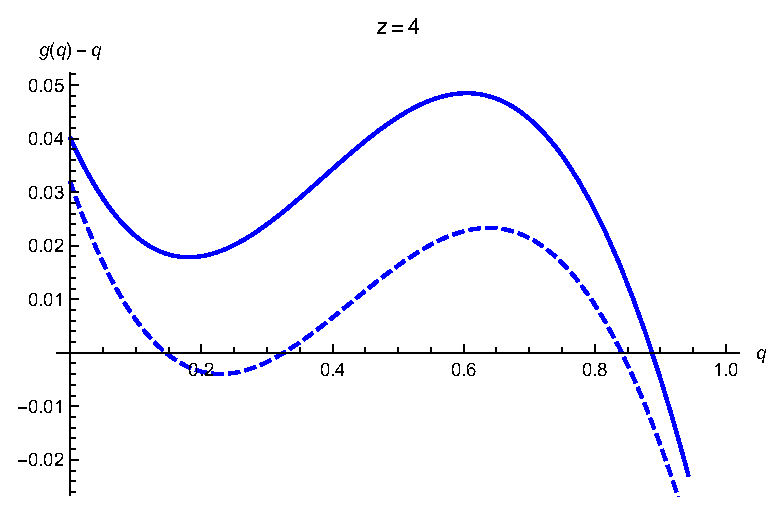
\includegraphics[width=0.6\textwidth]{figures/single_layer_gq}
\caption{$g(q)-q$ for parameters $z=4$;  sold is $r=0.35$, dashed is $r=0.371$}
\end{figure}

We are interested in the dynamics in the $\rho_0 \to 0$ limit and thus focus our attention on the dynamical behaviour of the recursion $q_{n+1} \leftarrow g(q_n)$. In particular, we would like to find the fixed points of the recursion and assess its stability. Gleeson demonstrated that in certain regimes of parameter space $(z,r)$, there are multiple fixed points $q_\infty(z,r)$ and these fixed points display bifurcating behaviour. Here we reproduce several plots from Gleeson's paper. Let us consider several cross sections of the $q_\infty(z,r)$, where we fix the adoption threshold parameter $r$ and vary the mean degree of the network $z$.  At small values of $r$, we see a single stable fixed point, with $q_\infty$ smoothly increasing as we increase $z$. The growth of $q_\infty$ becomes rather steep in some region of $z$ and levels off to a value close to 1 at large values of $z$. At a critical value of $r$ multiple fixed points appear with alternating stability and we observe several saddle point bifurcations. Since we iterate $q$ from $q_0 \ll 1$, the system will always end up on the lowest possible branch. We observe that in some intermediate regime of the threshold parameter there are discontinuous upward and downward leaps between lower branches of $q_\infty$, where the infection is contained, and the upper branches, where the infection is extensive in the system. In the last plot where $r$ is large, iterating $q$ from $0$ will alway lead to system to the lower branch of $q_\infty$ and the infection will never be extensive.

\begin{figure}
    \centering
    \begin{subfigure}[b]{0.8\textwidth}
        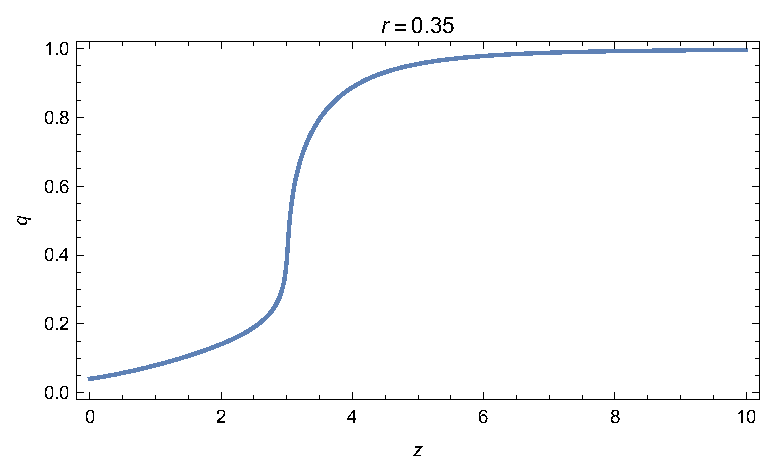
\includegraphics[width=\textwidth]{figures/one_layer_qz_r035}
    \end{subfigure}
    ~ %add desired spacing between images, e. g. ~, \quad, \qquad, \hfill etc.
      %(or a blank line to force the subfigure onto a new line)
    \begin{subfigure}[b]{0.8\textwidth}
        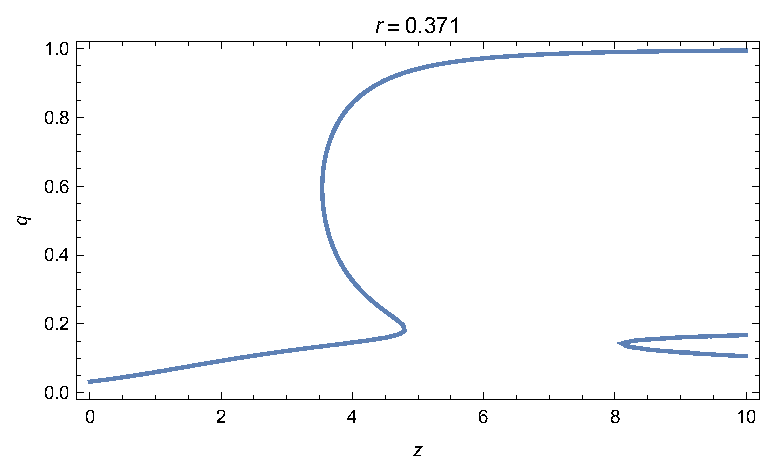
\includegraphics[width=\textwidth]{figures/one_layer_qz_r0371}
    \end{subfigure}
    ~ %add desired spacing between images, e. g. ~, \quad, \qquad, \hfill etc.
    %(or a blank line to force the subfigure onto a new line)
    \begin{subfigure}[b]{0.8\textwidth}
        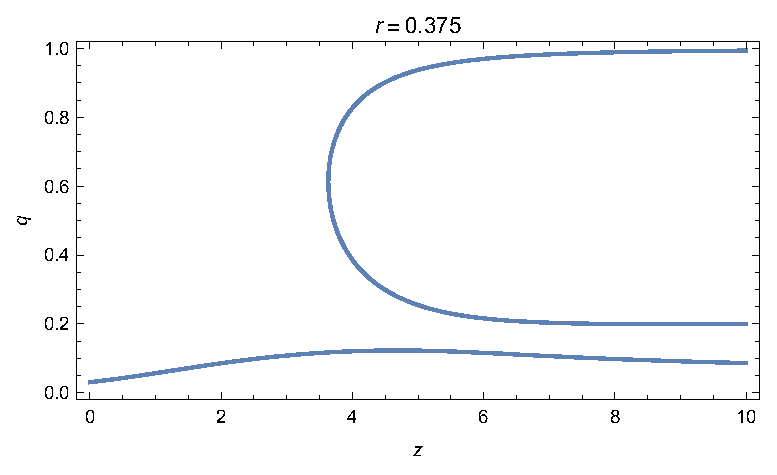
\includegraphics[width=\textwidth]{figures/one_layer_qz_r0375}
    \end{subfigure}
    \caption{Fixed point plot for increasing $r$. Note Goldilocks zone in middle figure.}
\end{figure}



These plots allow us to make a succinct qualitative summary of the effects of network topology and agent thresholds on the spread of ideas in a population of individuals. In the low threshold regime, the increase in network connectivity aids the spread of ideas, while in the intermediate threshold regime there is a `goldilocks zone' of values of $z$ where ideas can cascade extensively across the population; on either side of agents are either too sparsely connected for the contagion to become extensive or are become overly constrained by the influence of its neighbours too spark an initial adoption. Finally, if the threshold parameter is too large, then the infection will never cascade extensively because agents in the neighbourhood of the few available innovators are too constrained by other neighbours to adopt new ideas. Fixing $z$ across the plots, we observe that as $r$ is increased, a fixed point may drop discontinuously from the upper branch to the lower branch at some critical value of $r$.



In the duplex system, we follow the extension on Gleeson's work by Brummitt. We have a joint distribution for the degrees in both layers $p(\vb{k}) = p(k, k')$, where $k$ denotes the degree in the social network and $k'$ denotes the degree in the dependency network. In the case where the nodes in the social network are swapped to produce the dependency network $p(\vb{k}) \to p(k)p(k')$ in the limit of a large number of swaps; by effectively relabelling the nodes in the network, given a sufficiently large number of nodes, the degree of a node in the dependency network would be uncorrelated with it's degree in social network. In the case where the edges are swapped, the degree in the dependency network is preserved, hence $p(\vb{k}) \to p(k)\delta_{k,k'}$ in the large number of swap limit.

Let $F(\vb{m}, \vb{k})$ be the response function. To simplify the analysis, we assume the threshold for the transfer of awareness in the social network and the threshold for coordination in the dependency network are independently drawn from $\mathcal{N}(r, 0.2)$; hence the response function, which is the probability that the thresholds of the node is below $m/k$ and $m'/k'$ in both networks, is simply
\begin{equation}
F(\vb{m}, \vb{k}) = \Phi\qty(m/k)\Phi\qty(m'/k')
\end{equation}
where $\Phi$ is the cumulative distribution function for the normal distribution:
\begin{equation}
\Phi(x) = \int_{-\infty}^x \frac{1}{\sqrt{2\pi \sigma}} \exp\qty(-\frac{(x-r)^2}{2\sigma^2}).
\end{equation}
In the duplex situation, we have the expression for final infection fraction
\begin{equation}
\rho = \rho_0 + (1-\rho_0) \sum_{\vb{k}=0}^{\infty}p(\vb{k})\sum_{m=0}^k\sum_{m=0}^{k'}B^{k}_m(q_\infty)B^{k'}_{m'}(q'_\infty)F(\vb{m}, \vb{k})
\end{equation}
where $\vb{q}_\infty = (q_\infty, q'_\infty)$ is the fixed point of the recursive iteration
\begin{equation}
\vb{q}_{n+1} = \vb{g}(\vb{q}_n).
\end{equation}
and the function $\vb{g}(\vb{q}) = (g(\vb{q}), g'(\vb{q}) )$ is defined to be
\begin{align}
g(\vb{q}) &= \rho_0 + (1-\rho_0) \sum_{k=1}^\infty \sum_{k'=0}^\infty\frac{k}{z}p(\vb{k}) \sum_{m=0}^{k-1}\sum_{m'=0}^{k'}B^{k-1}_m(q)B^{k'}_{m'}(q')F(\vb{m}, \vb{k})\\
g'(\vb{q}) &= \rho_0 + (1-\rho_0) \sum_{k'=1}^\infty \sum_{k=0}^\infty\frac{k'}{z}p(\vb{k}) \sum_{m'=0}^{k'-1}\sum_{m=0}^{k}B^{k'-1}_m(q')B^{k}_{m}(q)F(\vb{m}, \vb{k})
\end{align}
Since we have assumed that the response thresholds in both layers are drawn from the same distribution, and by doing so making $F(\vb{m}, \vb{k})$ symmetric in the variables both network layers, we observe that
\begin{equation}
g(q, q') = g'(q', q).
\end{equation}
Thus if we assume $q_0 = q'_0 = \rho_0$, we have $q_n = q_n'$ for all $n$, and we only need to concern ourselves with one equation:
\begin{equation}
g(q) = g(q, q) = \rho_0 + (1-\rho_0) \sum_{k=1}^\infty \sum_{k'=0}^\infty\frac{k}{z}p(\vb{k}) \sum_{m=0}^{k-1}\sum_{m'=0}^{k'}B^{k-1}_m(q)B^{k'}_{m'}(q)F(\vb{m}, \vb{k}).
\end{equation}
Moreover the fact that $F(\vb{m}, \vb{k})$ is separable into  $F(\vb{m}, \vb{k}) = \Phi\qty(m/k)\Phi\qty(m'/k')$, we can make one final simplification:
\begin{align}
\rho &= \rho_0 + (1-\rho_0) \sum_{\vb{k}=0}^{\infty}p(\vb{k})\qty(\sum_{m=0}^k B^{k}_m(q_\infty)\Phi\qty(m/k))^2 \\
g(q) &= \rho_0 + (1-\rho_0) \sum_{k=1}^\infty \sum_{k'=0}^\infty\frac{k}{z}p(\vb{k}) \qty(\sum_{m=0}^{k-1}B^{k-1}_m(q)\Phi\qty(m/k))\qty(\sum_{m'=0}^{k'}B^{k'}_{m'}(q)\Phi\qty(m'/k')).
\end{align}
\begin{figure}
\centering
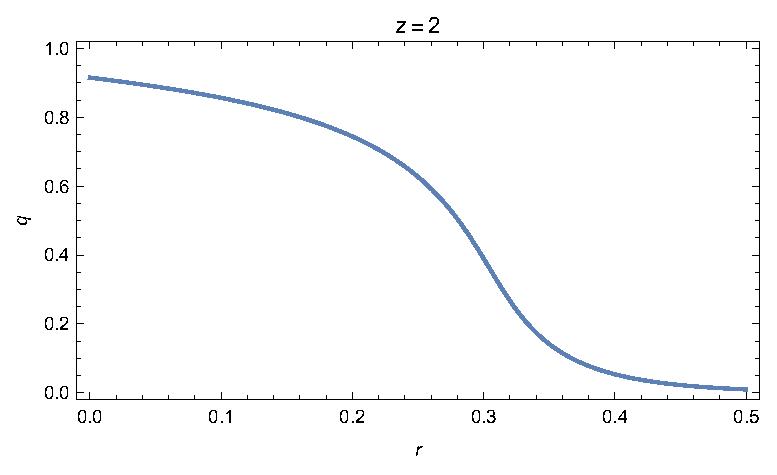
\includegraphics{figures/one_layer_qr_z2}
\end{figure}


\section{Simulations}

\newpage
\section{Conclusions}


\printbibliography
\end{document}
